\chapter{System Design}
\section{Architecture}

\begin{figure}[ht]
    \centering
    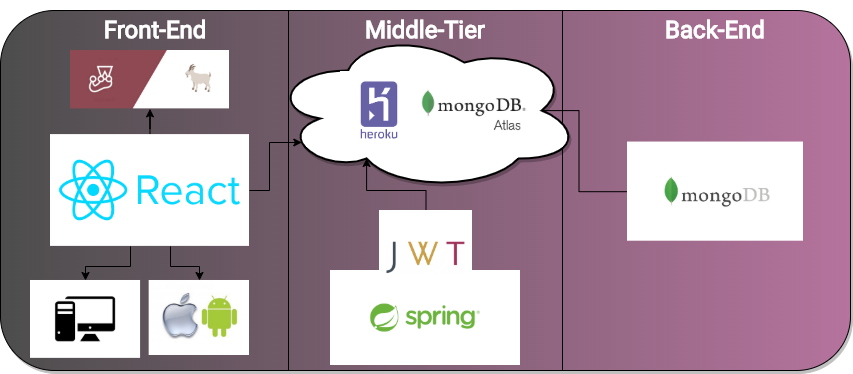
\includegraphics[scale=0.35]{Images/Project Architecture.png} 
    \label{proj_label}
    \caption{Project architecture diagram}
\end{figure}

The architecture (Figure ~\ref{proj_label}) of this project is comprised of three different tiers.
\begin{enumerate}
    \item The \textbf{Front-End} consists of the React application and of course all of the frameworks that go with it.
    \item The \textbf{Middle-tier} consists of my Spring Boot server which configures the REST API endpoints as well as the JWT API. These API's are of course, also hosted on Heroku and are in use by the front-end application to make requests.
    \item Lastly the \textbf{Back-End} which acts as a data tier includes a MongoDB database which stores all of the job details. I deployed the database on MongoDB Atlas to ensure the data is always available.
\end{enumerate}
In the following sections I will detail the design for each tier and explain why I made the decisions I did.

\section{Front End}
As this section contains the user interface, the only part of the application that the end user will actually see, I will go into extensive detail on it and provide many screenshots of each page and feature as well as provide some code snippets on how each feature was implemented.

\subsection{Login Page}
The login page (Figure ~\ref{login_label}) is the first page the user sees when they use my application. They cannot progress to any other pages in my application as all routes are authenticated. It consists of two text-boxes for entering user credentials, as well as a Bootstrap button for beginning the login sequence. If a user enters incorrect credentials they are alerted via a 'Bootstrap alert'. Further down the page there is a 'jumbotron' for styling purposes.

\begin{figure}[ht]
    \centering
    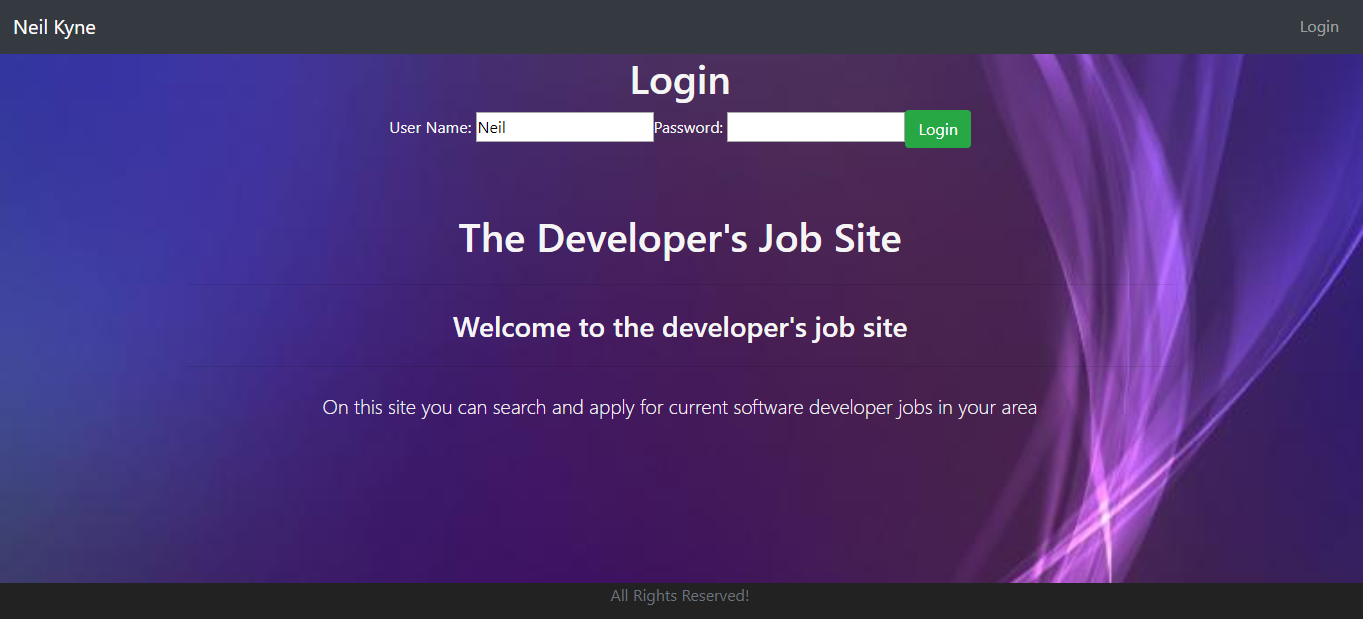
\includegraphics[scale=0.3]{Images/login.png} 
    \label{login_label}
    \caption{Login page}
\end{figure}

\subsection{Header \& Footer}
There is a navigation bar (Figure ~\ref{header_label}) at the top of every page in my application. This is useful for moving between pages and navigating the site. All routes in my application are authenticated meaning they cannot be accessed unless the user is logged in. Beginning from the left, it is comprised of;

\begin{figure}[ht]
    \centering
    
\includegraphics[scale=0.35]{Images/header.png} 
    \label{header_label}
    \caption{My 'navbar' at the top of every page}
\end{figure}
\begin{itemize}
    \item 'Neil Kyne' - This is a clickable link which simply takes the user to my GitHub profile.
    \item 'Home' - This brings the user to the home page.
    \item 'Jobs' - This brings the user to the full list of jobs.
    \item 'Logout' - This signs a user out and returns them to the login page.
\end{itemize}
Finally, just like the header, there is a footer at the bottom of every web-page. This just contains a generic 'All Rights Reserved' statement.

\subsection{Home Page}
The home page (Figure ~\ref{home_label}) is the core of the front-end application. It consists of four components:

\begin{figure}[ht]
    \centering
    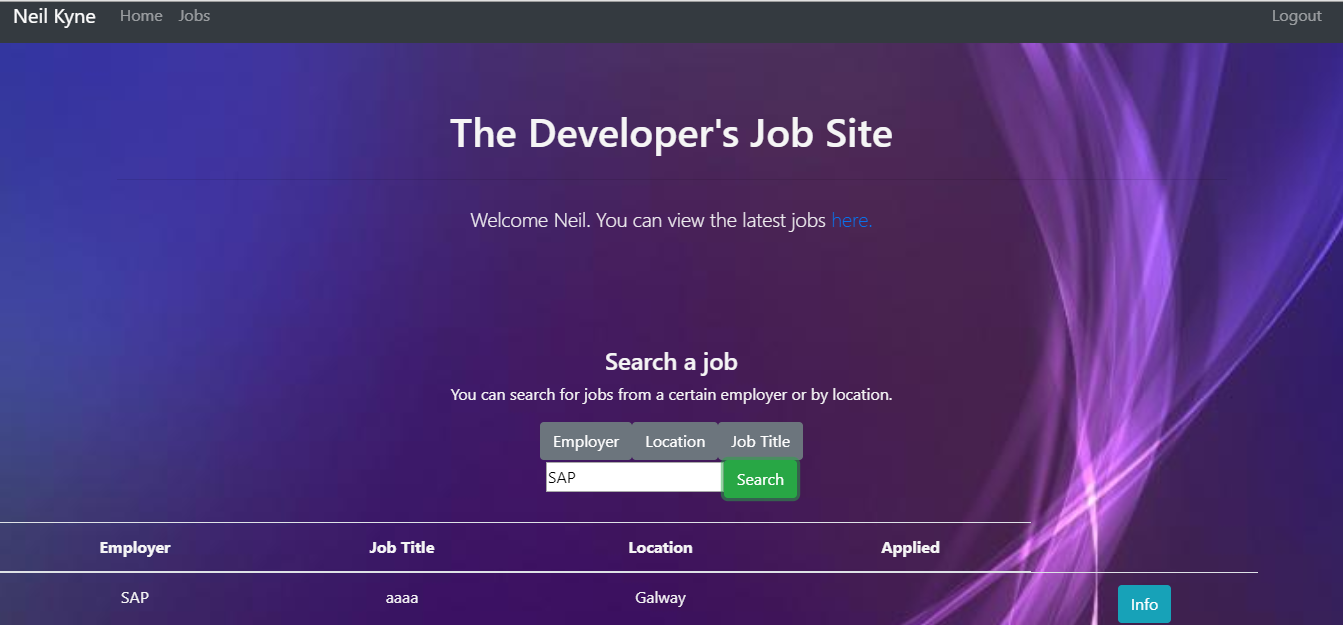
\includegraphics[scale=0.3]{Images/home.png} 
    \label{home_label}
    \caption{Home page}
\end{figure}

\subsubsection{1. Home Component}
This component simply acts as a greeting to the user. It comprises of a 'jumbotron' containing a welcome message for the user as well as a link to the full list of jobs.

\subsubsection{2. Search Component}
This component handles dynamic searching of jobs by their employer, location or job title.

\subsubsection{3. Results Component}
Here the results from the 'SearchComponent' are passed in as props to be displayed in a regular HTML table. Each row in the table has a 'View' button which opens up a Bootstrap 'Modal'.

\subsubsection{Apply Component}
This component (Figure ~\ref{apply_label}) is a 'modal' that displays more details about the job as well as gives an option to the user to apply for the job. If the user applies for that job they are notified via a Bootstrap alert and a marker is left beside the job in the table.

\begin{figure}[ht]
    \centering
    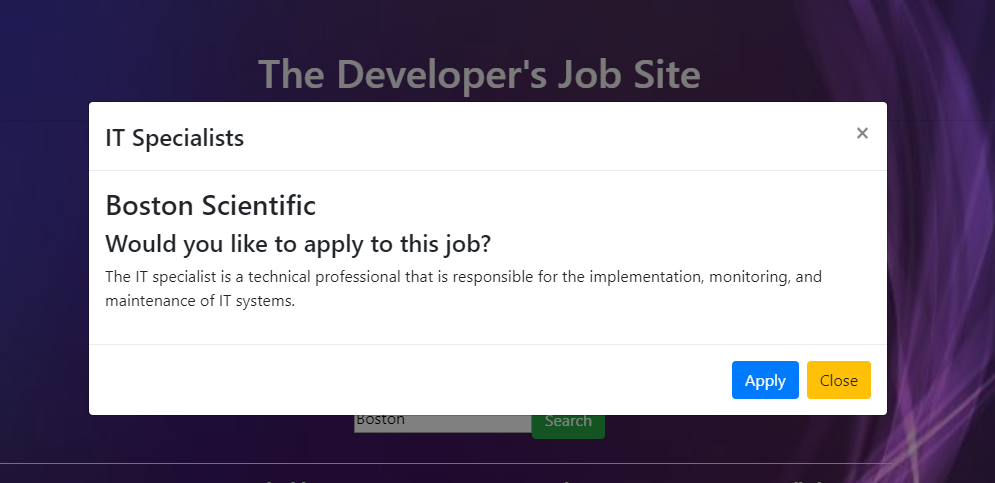
\includegraphics[scale=0.4]{Images/apply.png} 
    \label{apply_label}
    \caption{Apply modal}
\end{figure}

\subsection{Jobs Page}
This page (Figure ~\ref{jobs_label}) contains a 'Add' button which brings the user to the 'UpdateJobComponent'. The page also contains a table listing all the jobs in the database as well as two buttons in every row;

\begin{itemize}
    \item The \textbf{Delete button} removes a job listing from the database and refreshes the page.
    \item The \textbf{Update button} brings the user to the update job component.
\end{itemize}
\begin{figure}[ht]
    \centering
    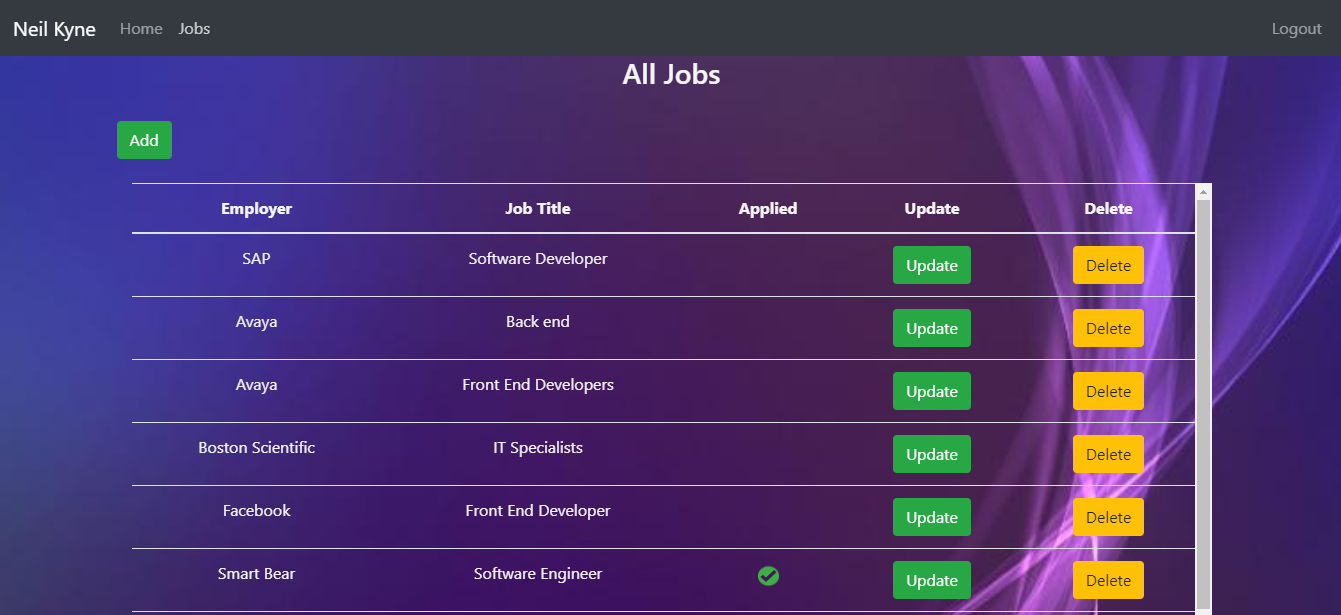
\includegraphics[scale=0.3]{Images/jobs.png} 
    \label{jobs_label}
    \caption{Jobs page}
\end{figure}

\subsection{Update/Create Job Page}
This page (Figure ~\ref{update_label}) acts as a two in one. If the user clicks on the update button in the 'ListJobsComponent' then the job details are passed in as props to this child component and the user can edit them. However if the user clicks on the add button in the previous component it will display an empty form for the user to fill in job details.

The form containing the job details is a React framework called 'Formik'. This is useful package that simplifies handling user data in React.

Lastly, the page has two buttons;
\begin{itemize}
    \item The \textbf{Save button} validates the form details, in my case it checks minimum character lengths in some of the text boxes. If they do not pass it displays a Bootstrap alert prompting the user to amend their mistake. If they pass validation it returns the user to the Jobs Page.
    \item The \textbf{Back button} returns the user to the previous page and discards any changes to the job.
\end{itemize}
\begin{figure}[ht]
    \centering
    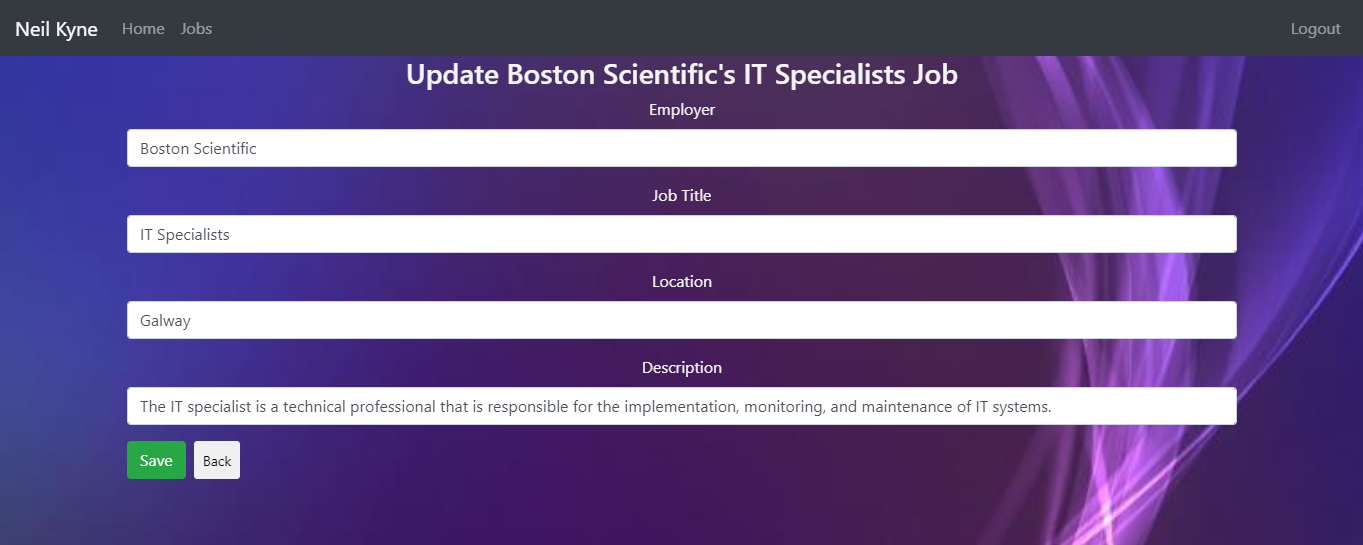
\includegraphics[scale=0.3]{Images/update.png} 
    \label{update_label}
    \caption{Update page}
\end{figure}

\section{Middle Tier}
This section consists of a lot of the logic and actual computation in my application. The most important part of this tier is of course the REST API. This is what the front-end communicates with to manipulate or remove data. This tier also contains a JWT API which allows users to request new tokens and prove authentication. Both of these API's are hosted on Heroku.

\subsection{Spring Boot Project Structure}
The REST API hosted on Heroku was built using Spring Boot. In this section I will summarize my project setup (Figure ~\ref{setup_label}) and design for building the API.

\begin{figure}[ht]
    \centering
    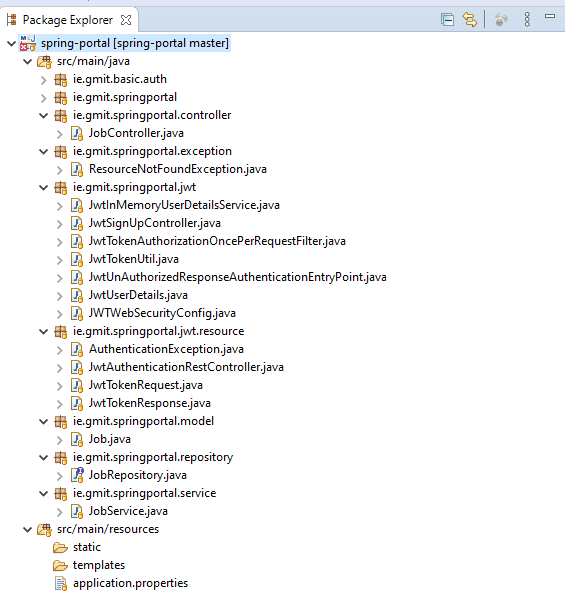
\includegraphics[scale=0.7]{Images/setup.png} 
    \label{setup_label}
    \caption{Project structure}
\end{figure}
%Might want to go into more detail on these..
\paragraph{My Boot project consists of four main packages;}
\begin{figure}[ht]
    \centering
    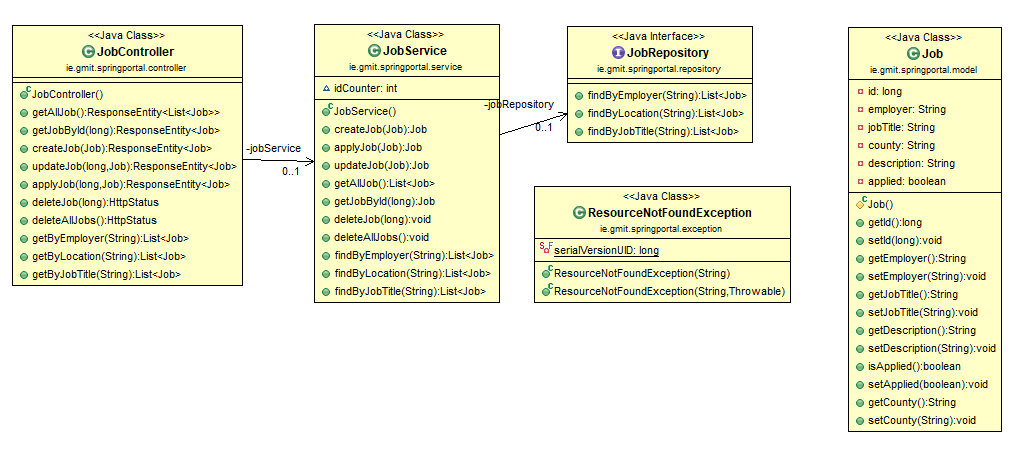
\includegraphics[scale=0.4]{Images/API UML.png} 
    \label{api_label}
    \caption{UML diagram of my API}
\end{figure}
\begin{itemize}
    \item The \textbf{Model} package describes the model that we want to work with, in this case a job. This is what is persisted to the MongoDB database and what is displayed at our front-end.
    \item The \textbf{Repository} package configures the MongoDB repository. The 'JobRepository' is used for accessing data from the database. It automatically implements all the basic CRUD operations one might want to perform on a database, I also added three custom methods for searching (Figure ~\ref{repo_label}). Spring Boot tries to auto-configure most of the stuff for you based on the dependencies that you have added in the pom.xml file.
    Since I added a 'spring-boot-starter-data-mongodb' dependency, Spring Boot automatically tries to build a connection with MongoDB by reading the database configuration from the 'application.properties' file.
    \begin{figure}[h]
    \centering
    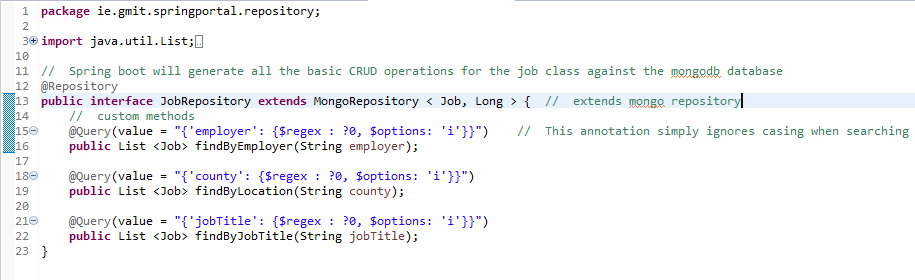
\includegraphics[scale=0.5]{Images/repo.png} 
    \label{repo_label}
    \caption{Mongo repository}
    \end{figure}
    \item The \textbf{Service} package describes the service layer. This package contains a lot of the business logic. The 'JobService' class connects with the 'JobRepository' class to perform CRUD operations on the database.
    \item Finally the \textbf{Controller} package contains the 'JobController' class. This is the API which will be exposed to the front-end users.
\end{itemize}


Aside from the listed packages there are;
\begin{itemize}
    \item A \textbf{Basic Authentication} package which is no longer in use as I now use JWT authentication.
    \item An \textbf{Exception} package for handling exceptions or errors with requests to the API.
    \item Two \textbf{JWT} packages.
        \begin{itemize}
            \item The resource package contains the resources related to the REST API and most importantly the 'JWTAuthenticationRestController'. This is the API we send requests to to receive JWT tokens.
            \item The JWT package contains all of the actual logic for creating the JWT token and the user details required to do so.
        \end{itemize}
        \begin{figure}[ht]
        \centering
        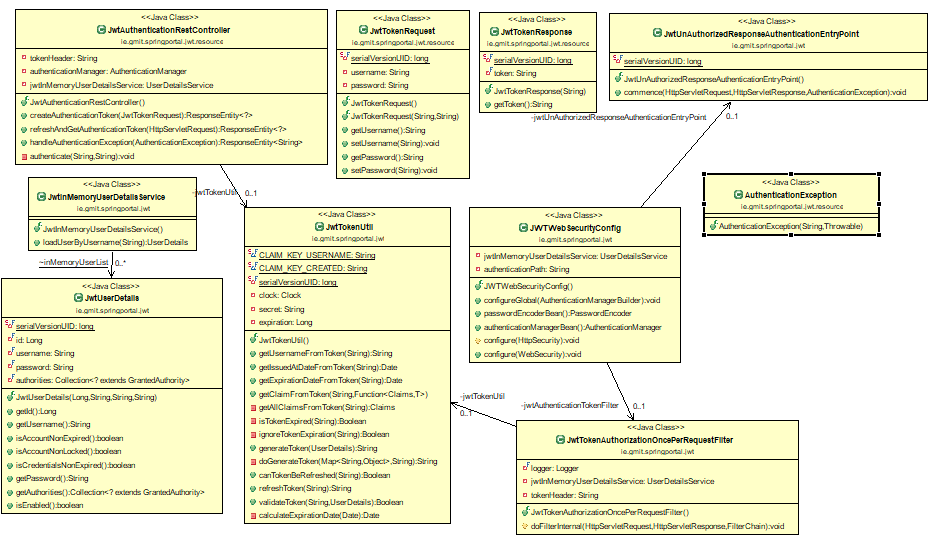
\includegraphics[scale=0.4]{Images/JWT UML.png} 
        \label{jwtuml_label}
        \caption{UML diagram for JWT packages}
        \end{figure}
        \item The \textbf{pom.xml} file contains project information and configuration information for maven to build the project such as dependencies, build directory and source directories. Maven reads the pom.xml file, then executes the goal \cite{POM}. Here (Figure ~\ref{pom_label}) I specified many dependencies to aid in building the API.
        \item Lastly, the \textbf{application.properties} file is used to keep project properties in a single file to run the application in a different environment.
\end{itemize}
\begin{figure}[ht]
    \centering
    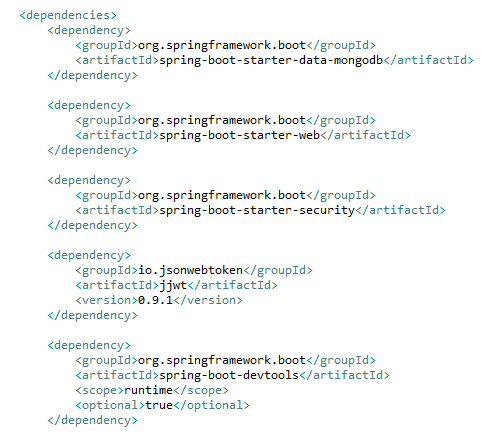
\includegraphics[scale=0.6]{Images/pom.png} 
    \label{pom_label}
    \caption{pom.xml file declaring dependencies}
\end{figure}

\subsection{Heroku}
In order for the React application to be able to access the API's online they would have to be hosted online. For this I used Heroku. To create an empty Heroku application via the Heroku Command Line Interface (CLI) I ran:

\begin{verbatim}
heroku create spring-portal-api
\end{verbatim}
To deploy the REST API to Heroku I first initialized a Git repository in my 'spring-portal' directory.

\begin{verbatim}
git init
\end{verbatim}
I then update the index using the current content found in the working tree, to prepare the content staged for the next commit.

\begin{verbatim}
git add .
\end{verbatim}
This stores the current content of the index in a new commit along with a message from the user describing the changes.

\begin{verbatim}
git commit -m "Added API to Heroku"
\end{verbatim}
Finally, to push to the new Heroku repository you use:

\begin{verbatim}
git push heroku master
\end{verbatim}

\section{Back-End}
The back-end tier stores all of my job data. I deployed my database online using MongoDB Atlas. This makes it available at all times to the API.

\subsection{MongoDB Atlas}
There were a number of steps required to deploy my database on Atlas.

\begin{enumerate}
    \item Create a MongoDB Atlas account.
    \item Create a free tier cluster by clicking "Build a new cluster". From here choose a cloud provider and region. Finally Choose the free tier cluster option, selecting the M0 sandbox (free tier) and name your cluster.
    \begin{itemize}
        \item Atlas Free Tier clusters provide a small-scale development environment to host your data. Free Tier clusters never expire, and provide access to a subset of Atlas features and functionality \cite{Atlas}.
    \end{itemize}
    \item Next, when the cluster is created, click 'Connect'. Here we white-list our IP address. Secondly, add yourself as a database user admin to allow for full access.
    \item Now we are ready to connect the cluster to the Spring Boot project. Click connect, configure the project settings and copy the string (Figure ~\ref{atlas1_label}).
    \item Head over to the 'application.properties' file and paste in the string, replacing the blank username and password with your own.
\end{enumerate}

\begin{figure}[h]
    \centering
    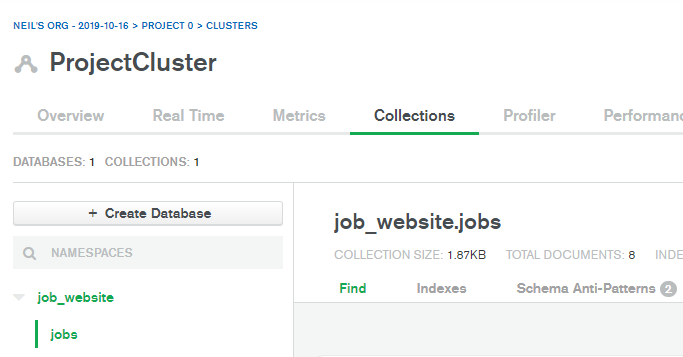
\includegraphics[scale=0.37]{Images/atlas2.png}
    \label{atlas2_label}
    \caption{Database with its 'jobs' collection}
\end{figure}
\begin{figure}[ht]
    \centering
    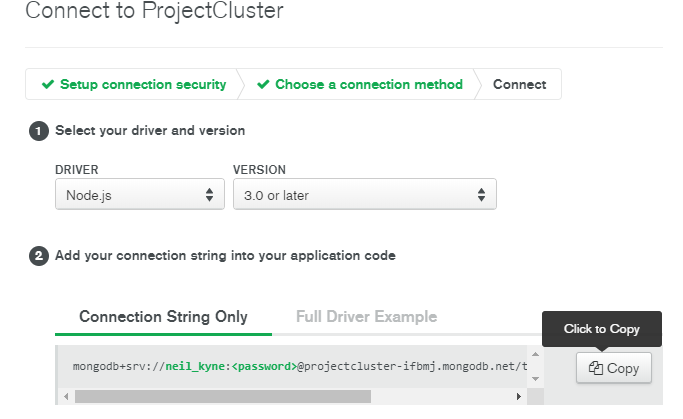
\includegraphics[scale=0.5]{Images/atlas.png} 
    \label{atlas1_label}
    \caption{Application connection string}
\end{figure}

It may have been noticed I never specified a name for the database or a name for the collection anywhere on MongoDB Atlas. All of this is configured in my Spring Boot application. I specify these details using the Spring data annotations provided for use with MongoDB. I also specify a few other settings for the 'Job' documents using these annotations (Figure ~\ref{atlas3_label}) such as the \textbf{@Id} of the document which is the identifier for every mongo document, as well as more basic annotations such as \textbf{@NotBlank} which forbids empty values and \textbf{@Size} which allows a user to set a max input size.

I define the collection name in the database above the class declaration with \textbf{@Document(collection = "jobs")}. Finally the database name is declared in the 'application.properties' file with \newline \textbf{spring.data.mongodb.database=job\_website}.

\begin{figure}[ht]
    \centering
    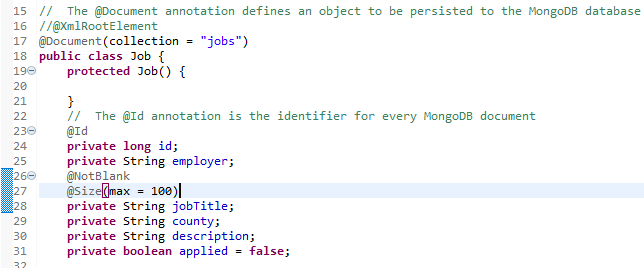
\includegraphics[scale=0.5]{Images/atlas3.png}
    \label{atlas3_label}
    \caption{Job model outlining some mongo configurations using Spring-Mongo annotations.}
\end{figure}

